\documentclass[a4paper,12pt]{article}
\usepackage{float}
\usepackage[table]{xcolor} % Para colorir as linhas da tabela
%\usepackage{array} % Para melhorar a formatação de tabelas
\usepackage[brazil]{babel}
\usepackage{diagbox}
\usepackage{amsmath}
\usepackage{amssymb}
\usepackage{multirow}
\usepackage{pdfpages}
\usepackage{multicol}
\usepackage{graphicx}
%\usepackage{animate}
%\usepackage{tabularx}
\usepackage[font=footnotesize, labelfont=bf, listformat=empty]{caption}
\usepackage{geometry}
\usepackage{listings}
\usepackage{fontspec}
\usepackage{minted}
\usepackage{lastpage}
%\usepackage{subcaption}
\usepackage[skins,xparse,breakable]{tcolorbox}
%\usepackage{longtable}
\usepackage{titlesec}
\usepackage{fancyhdr}
\usepackage{ragged2e}
\usepackage{setspace}
\usepackage{booktabs}
\usepackage{siunitx}
\usepackage{enumitem}
\usepackage{minted}
\usepackage[colorlinks=true, allcolors=black]{hyperref}
\usepackage{tikz}

\sisetup{
    output-decimal-marker = {,},
    table-number-alignment = center
}
\usetikzlibrary{karnaugh}
\usetikzlibrary{positioning,arrows.meta,shapes.multipart,calc}

%\usetikzlibrary{arrows,shapes,automata,positioning,calc}
% Configurações de margens e espaçamento
\geometry{a4paper, left=2.5cm, right=2.5cm, top=2.5cm, bottom=2cm}
\onehalfspacing

% Configurações de títulos
\titleformat{\section}{\normalfont\Large\bfseries}{\thesection}{1em}{}
\titleformat{\subsection}{\normalfont\large\bfseries}{\thesubsection}{1em}{}
\titleformat{\subsubsection}
  {\normalfont\large}
  {\textbf{\thesubsubsection}}
  {0.25em}{}

\setcounter{tocdepth}{3}
\newcommand{\cod}[1]{\texttt{#1}}

\renewcommand{\listingscaption}{Código}
\newenvironment{code}{\captionsetup{type=listing}}{}

% Configurações de cores
\definecolor{LightSeaGreen}{rgb}{0.1255, 0.6980, 0.6667}
\definecolor{whitesmoke}{rgb}{0.96, 0.96, 0.96}
\definecolor{cinza}{RGB}{160, 160, 160}
\definecolor{cinza_claro}{RGB}{240, 240, 240} % Cinza claro

\newtcolorbox{codebox}[1]{
    title=#1,
    fonttitle=\small\bfseries,
    colback=blue!2.5!white,
    colframe=blue!62!white,
    arc=2pt,
    boxrule=0.8pt,
    left=4pt,
    right=4pt,
    top=4pt,
    bottom=4pt,
    breakable,
    enhanced jigsaw
}

\setminted[asm]{
    fontsize=\scriptsize,
    style=manni,
    linenos=true,
    breaklines=true,
    mathescape=true,
    bgcolor=cinza_claro,
    breakanywhere=true,
}

\newcommand{\hex}[1]{\textcolor{green!50!black}{#1}}

% Configurações de cabeçalho e rodapé
\pagestyle{fancy}
\fancyhf{}
\fancyhead[L]{\footnotesize{Relatório do Laboratório 4}}
\fancyhead[R]{\footnotesize{2025/2 - Turma 02}}
\fancyfoot[R]{\footnotesize{Página \hspace{0.05cm} \thepage \hspace{0.05cm} de \pageref{LastPage}}}
\fancyfoot[L]{\footnotesize{Organização e Arquitetura de Computadores - CIC0099}}

% Adiciona uma linha preta acima do rodapé
\renewcommand{\footrulewidth}{0.4pt} % Espessura da linha
\renewcommand{\footrule}{\vbox to 0pt{\hrule width \textwidth height \footrulewidth \vss}} % Desenha a linha

% Novo Comando para chamar a capa
\newcommand{\capa}{
    \begin{titlepage}
        \begin{multicols}{2}
            \begin{flushleft}
                
\includegraphics[width=0.45\linewidth]{Recursos/Imagens/UnB_logo.png}
            \end{flushleft}
            \columnbreak
            \begin{flushright}
                Universidade de Brasília \\
                Instituto de Exatas \\
                Departamento de Ciência da Computação
            \end{flushright}
        \end{multicols}
        \begin{center}
        \vspace{-20pt}
        \rule{\textwidth}{0.4pt}
        \end{center}
        \vspace{0.6cm}
        \begin{center}
            {\Huge \textbf{Relatório do Laboratório 4}} \\[0.5em]
            {\Huge \textbf{Processador Pipeline}} \\ [0.5em]
            {\large CIC0099 - Organização e Arquitetura de Computadores} \\[0.25em]
            {\large Turma 02 - Prof. Dr. Ricardo Pezzuol Jacobi} \\
            \vfill
            {\Large \textbf{Grupo B4}} \\
            \begin{table}[H]
                \centering
                \begin{tabular}{l r}
                    Henrique Morcelles Salum & 232003008 \\
                    Athos Calixto Muniz & 211068261 \\
                    Gabriela Fernanda Rodrigues Costa & 180120859 \\
                    Cauê Araújo Euzebio & 211028195 \\
                    Lucas Silva Nóbrega & 180035096
                \end{tabular}
                \label{tab:placeholder}
            \end{table}
        \end{center}
    \end{titlepage}
}

\begin{document}

\capa

% Sumário
\newpage
\tableofcontents
\newpage

\section{Introdução}
O presente experimento tem como objetivo introduzir os alunos ao processo de projeto e implementação de sistemas digitais utilizando VHDL como Linguagem de Descrição de Hardware (HDL). O laboratório busca promover o treinamento prático em modelagem, análise e síntese de circuitos digitais, utilizando o ambiente de desenvolvimento \textbf{Intel Quartus Prime v24.1}.

Como aplicação prática, propõe-se a implementação de um processador Pipeline compatível com a ISA RV32I reduzida, contendo as instruções: \cod{add}, \cod{sub}, \cod{and}, \cod{or}, \cod{slt}, \cod{lw}, \cod{sw}, \cod{beq}, \cod{jal}, \cod{jalr}, \cod{addi} e \cod{lui}. Essa abordagem permite compreender o funcionamento interno de um processador Pipeline.

A implementação será validada por meio de simulação funcional e temporal, com análise de \textit{timing} e frequência máxima de operação, permitindo compreender, de forma integrada, o funcionamento de uma arquitetura RISC-V.


\section{Métodos e Análise}

\subsection{Experimento}
\begin{tcolorbox}[title=Enunciado, colback=blue!5!white, colframe=blue!75!black]
Implemente o processador Pipeline com ISA Reduzida com as instruções: \cod{add}, \cod{sub}, \cod{and}, \cod{or}, \cod{slt}, \cod{lw}, \cod{sw}, \cod{beq}, \cod{jal}, e ainda as instruções \cod{jalr}, \cod{addi} e \cod{lui}.
\end{tcolorbox}

Para realizar o solicitado, é-nos fornecido o esquemático de uma implementação do Pipeline com ISA reduzida. Nesse esquemático, porém, foi necessário realizar alterações no caminho de dados, que serão devidamente justificadas adiante.

\begin{figure}[H]
    \centering
    % Important: If latex complains about unicode characters,
% please use "\usepackage[utf8x]{inputenc}" in your preamble
% You can change the size of the picture by putting it into the construct:
% 1) \resizebox{10cm}{!}{"below picture"} to scale horizontally to 10 cm
% 2) \resizebox{!}{15cm}{"below picture"} to scale vertically to 15 cm
% 3) \resizebox{10cm}{15cm}{"below picture"} a combination of above two
% It is not recomended to use the scale option of the tikzpicture environment.
\resizebox{\textwidth}{!}{
\begin{tikzpicture}[x=1pt,y=-1pt,line cap=rect]
\def\logisimfontA#1{{\fontspec{Arial Rounded MT Bold}#1}}
\def\logisimfontB#1{{\fontspec{Arial Rounded MT Bold}#1}}
\def\logisimfontC#1{{\fontspec{Arial Rounded MT Bold}#1}}
\def\logisimfontD#1{{\fontspec{Arial Rounded MT Bold}#1}}
\definecolor{custcol_3c_d9_ff}{RGB}{60, 217, 255}
\definecolor{custcol_a8_a8_a8}{RGB}{168, 168, 168}
\definecolor{custcol_87_87_87}{RGB}{135, 135, 135}
\definecolor{custcol_0_0_0}{RGB}{0, 0, 0}
\definecolor{custcol_ff_ff_ff}{RGB}{255, 255, 255}
\draw [line width=4.0pt, custcol_0_0_0 ]  (915.0,446.0) -- (965.0,446.0) ;
\draw [line width=3.0pt, custcol_0_0_0 ]  (55.0,376.0) -- (55.0,456.0) ;
\draw [line width=4.0pt, custcol_0_0_0 ]  (75.0,346.0) -- (105.0,346.0) ;
\draw [line width=4.0pt, custcol_0_0_0 ]  (835.0,306.0) -- (965.0,306.0) ;
\draw [line width=4.0pt, custcol_0_0_0 ]  (715.0,306.0) -- (745.0,306.0) -- (815.0,306.0) ;
\draw [line width=4.0pt, custcol_0_0_0 ]  (715.0,426.0) -- (745.0,426.0) -- (815.0,426.0) ;
\draw [line width=3.0pt, custcol_3c_d9_ff ]  (745.0,106.0) -- (815.0,106.0) ;
\draw [line width=3.0pt, custcol_3c_d9_ff ]  (745.0,66.0) -- (815.0,66.0) ;
\draw [line width=3.0pt, custcol_3c_d9_ff ]  (733.0,26.0) -- (815.0,26.0) ;
\draw [line width=4.0pt, custcol_0_0_0 ]  (835.0,426.0) -- (865.0,426.0) -- (865.0,516.0) -- (1065.0,516.0) ;
\draw [line width=3.0pt, custcol_3c_d9_ff ]  (1345.0,96.0) -- (1375.0,96.0) ;
\draw [line width=3.0pt, custcol_3c_d9_ff ]  (1085.0,96.0) -- (1235.0,96.0) -- (1235.0,336.0) ;
\draw [line width=4.0pt, custcol_0_0_0 ]  (195.0,136.0) -- (245.0,136.0) ;
\draw [line width=4.0pt, custcol_0_0_0 ]  (835.0,496.0) -- (935.0,496.0) -- (935.0,236.0) ;
\draw [line width=4.0pt, custcol_0_0_0 ]  (835.0,546.0) -- (1065.0,546.0) ;
\draw [line width=4.0pt, custcol_0_0_0 ]  (1345.0,446.0) -- (1395.0,446.0) ;
\draw [line width=3.0pt, custcol_0_0_0 ]  (685.0,266.0) -- (685.0,286.0) ;
\draw [line width=4.0pt, custcol_0_0_0 ]  (835.0,526.0) -- (855.0,526.0) -- (855.0,466.0) -- (875.0,466.0) ;
\draw [line width=4.0pt, custcol_0_0_0 ]  (465.0,476.0) -- (815.0,476.0) ;
\draw [line width=4.0pt, custcol_0_0_0 ]  (245.0,176.0) -- (195.0,176.0) -- (195.0,216.0) -- (375.0,216.0) ;
\draw [line width=4.0pt, custcol_3c_d9_ff ]  (835.0,116.0) -- (865.0,116.0) -- (865.0,206.0) -- (905.0,206.0) ;
\draw [line width=3.0pt, custcol_3c_d9_ff ]  (1345.0,116.0) -- (1415.0,116.0) -- (1415.0,396.0) ;
\draw [line width=4.0pt, custcol_0_0_0 ]  (465.0,306.0) -- (595.0,306.0) ;
\draw [line width=4.0pt, custcol_0_0_0 ]  (465.0,346.0) -- (595.0,346.0) ;
\draw [line width=4.0pt, custcol_3c_d9_ff ]  (744.5,116.0) -- (815.0,116.0) ;
\draw [line width=3.0pt, custcol_3c_d9_ff ]  (1085.0,116.0) -- (1175.0,116.0) -- (1175.0,336.0) ;
\draw [line width=4.0pt, custcol_0_0_0 ]  (1045.0,376.0) -- (1065.0,376.0) ;
\draw [line width=4.0pt, custcol_0_0_0 ]  (1085.0,376.0) -- (1105.0,376.0) -- (1145.0,376.0) ;
\draw [line width=4.0pt, custcol_0_0_0 ]  (1085.0,236.0) -- (1325.0,236.0) ;
\draw [line width=4.0pt, custcol_0_0_0 ]  (1265.0,446.0) -- (1325.0,446.0) ;
\draw [line width=3.0pt, custcol_3c_d9_ff ]  (733.0,146.0) -- (785.0,146.0) -- (785.0,586.0) -- (55.0,586.0) -- (55.0,546.0) ;
\draw [line width=4.0pt, custcol_0_0_0 ]  (565.0,176.0) -- (555.0,176.0) -- (555.0,526.0) -- (815.0,526.0) ;
\draw [line width=4.0pt, custcol_0_0_0 ]  (495.0,86.0) -- (640.0,86.0) ;
\draw [line width=3.0pt, custcol_3c_d9_ff ]  (745.0,86.0) -- (815.0,86.0) ;
\draw [line width=3.0pt, custcol_3c_d9_ff ]  (740.0,46.0) -- (815.0,46.0) ;
\draw [line width=4.0pt, custcol_0_0_0 ]  (1345.0,286.0) -- (1365.0,286.0) -- (1365.0,406.0) -- (1395.0,406.0) ;
\draw [line width=4.0pt, custcol_3c_d9_ff ]  (1085.0,66.0) -- (1275.0,66.0) -- (1275.0,106.0) -- (1325.0,106.0) ;
\draw [line width=4.0pt, custcol_3c_d9_ff ]  (965.0,206.0) -- (1015.0,206.0) -- (1015.0,336.0) ;
\draw [line width=4.0pt, custcol_0_0_0 ]  (445.0,496.0) -- (415.0,496.0) -- (415.0,346.0) -- (415.0,86.0) -- (475.0,86.0) -- (485.0,86.0) ;
\draw [line width=4.0pt, custcol_0_0_0 ]  (195.0,216.0) -- (195.0,346.0) -- (175.0,346.0) ;
\draw [line width=3.0pt, custcol_3c_d9_ff ]  (835.0,106.0) -- (895.0,106.0) -- (895.0,416.0) ;
\draw [line width=4.0pt, custcol_3c_d9_ff ]  (835.0,76.0) -- (935.0,76.0) -- (935.0,106.0) -- (1065.0,106.0) ;
\draw [line width=4.0pt, custcol_0_0_0 ]  (395.0,216.0) -- (565.0,216.0) ;
\draw [line width=4.0pt, custcol_0_0_0 ]  (1085.0,516.0) -- (1145.0,516.0) ;
\draw [line width=4.0pt, custcol_3c_d9_ff ]  (835.0,36.0) -- (955.0,36.0) -- (955.0,66.0) -- (1065.0,66.0) ;
\draw [line width=4.0pt, custcol_0_0_0 ]  (335.0,346.0) -- (375.0,346.0) ;
\draw [line width=4.0pt, custcol_0_0_0 ]  (745.0,386.0) -- (745.0,426.0) ;
\draw [line width=4.0pt, custcol_0_0_0 ]  (745.0,306.0) -- (745.0,346.0) ;
\draw [line width=4.0pt, custcol_0_0_0 ]  (535.0,526.0) -- (555.0,526.0) ;
\draw [line width=4.0pt, custcol_0_0_0 ]  (195.0,346.0) -- (215.0,346.0) ;
\draw [line width=4.0pt, custcol_0_0_0 ]  (35.0,366.0) -- (25.0,366.0) -- (25.0,46.0) -- (625.0,46.0) -- (625.0,196.0) -- (605.0,196.0) ;
\draw [line width=4.0pt, custcol_0_0_0 ]  (465.0,496.0) -- (815.0,496.0) ;
\draw [line width=4.0pt, custcol_0_0_0 ]  (395.0,346.0) -- (415.0,346.0) -- (445.0,346.0) ;
\draw [line width=4.0pt, custcol_0_0_0 ]  (415.0,496.0) -- (415.0,526.0) -- (435.0,526.0) ;
\draw [line width=4.0pt, custcol_0_0_0 ]  (1105.0,376.0) -- (1105.0,286.0) -- (1325.0,286.0) ;
\draw [line width=4.0pt, custcol_0_0_0 ]  (865.0,426.0) -- (875.0,426.0) ;
\draw [line width=4.0pt, custcol_0_0_0 ]  (1345.0,536.0) -- (1365.0,536.0) -- (1365.0,606.0) -- (575.0,606.0) -- (575.0,386.0) -- (595.0,386.0) ;
\draw [line width=3.0pt, custcol_0_0_0 ]  (765.0,366.0) -- (775.0,366.0) -- (775.0,576.0) -- (75.0,576.0) -- (75.0,546.0) ;
\draw [line width=4.0pt, custcol_0_0_0 ]  (1435.0,426.0) -- (1455.0,426.0) -- (1455.0,616.0) -- (565.0,616.0) -- (565.0,426.0) -- (595.0,426.0) ;
\draw [line width=4.0pt, custcol_0_0_0 ]  (35.0,326.0) -- (5.0,326.0) -- (5.0,96.0) -- (335.0,96.0) -- (335.0,156.0) -- (285.0,156.0) ;
\fill [line width=4.0pt, custcol_0_0_0]  (195.0,346.0) ellipse (6.0 and 6.0 );
\fill [line width=4.0pt, custcol_0_0_0]  (415.0,496.0) ellipse (6.0 and 6.0 );
\fill [line width=4.0pt, custcol_0_0_0]  (555.0,526.0) ellipse (6.0 and 6.0 );
\fill [line width=4.0pt, custcol_0_0_0]  (1105.0,376.0) ellipse (6.0 and 6.0 );
\fill [line width=4.0pt, custcol_0_0_0]  (745.0,306.0) ellipse (6.0 and 6.0 );
\fill [line width=4.0pt, custcol_0_0_0]  (865.0,426.0) ellipse (6.0 and 6.0 );
\fill [line width=4.0pt, custcol_0_0_0]  (195.0,216.0) ellipse (6.0 and 6.0 );
\fill [line width=4.0pt, custcol_0_0_0]  (415.0,346.0) ellipse (6.0 and 6.0 );
\fill [line width=4.0pt, custcol_0_0_0]  (475.0,86.0) ellipse (6.0 and 6.0 );
\fill [line width=4.0pt, custcol_0_0_0]  (745.0,426.0) ellipse (6.0 and 6.0 );
\draw [line width=2.0pt, custcol_0_0_0 ]  (375.0,126.0) -- (394.0,126.0) ;
\draw [line width=2.0pt, custcol_0_0_0 ]  (395.0,126.0) -- (395.0,565.0) ;
\draw [line width=2.0pt, custcol_0_0_0 ]  (395.0,566.0) -- (376.0,566.0) ;
\draw [line width=2.0pt, custcol_0_0_0 ]  (375.0,566.0) -- (375.0,127.0) ;
\fill [line width=1.0pt, custcol_0_0_0]  (375.0,216.0) ellipse (2.0 and 2.0 );
\fill [line width=1.0pt, custcol_0_0_0]  (375.0,346.0) ellipse (2.0 and 2.0 );
\fill [line width=1.0pt, custcol_0_0_0]  (395.0,216.0) ellipse (2.0 and 2.0 );
\fill [line width=1.0pt, custcol_0_0_0]  (395.0,346.0) ellipse (2.0 and 2.0 );
\logisimfontB{\fontsize{20pt}{20pt}\fontseries{bx}\selectfont\node[inner sep=0, outer sep=0, custcol_0_0_0, anchor=base west] at  (610.0,366.0)  {Register};}
\logisimfontB{\fontsize{20pt}{20pt}\fontseries{bx}\selectfont\node[inner sep=0, outer sep=0, custcol_0_0_0, anchor=base west] at  (628.0,385.0)  {Bank};}
\draw [line width=1.0pt, custcol_0_0_0 ]  (680.0,446.0) -- (685.0,432.0) -- (690.0,446.0) ;
\begin{pgfpicture}
   \begin{pgfmagnify}{1pt}{-1pt}
      \pgfsetrectcap
      \pgfsetcornersarced{\pgfpoint{10.0}{10.0}}
      \pgfsetlinewidth{4.0}
      \color{custcol_0_0_0}
      \pgfsetfillopacity{1.0}
      \pgfpathrectanglecorners{\pgfpoint{595.0}{286.0}}{\pgfpoint{715.0}{446.0}}
      \pgfusepath{stroke}
   \end{pgfmagnify}
\end{pgfpicture}
\fill [line width=1.0pt, custcol_0_0_0]  (595.0,306.0) ellipse (2.0 and 2.0 );
\fill [line width=1.0pt, custcol_0_0_0]  (595.0,346.0) ellipse (2.0 and 2.0 );
\fill [line width=1.0pt, custcol_0_0_0]  (595.0,386.0) ellipse (2.0 and 2.0 );
\fill [line width=1.0pt, custcol_0_0_0]  (595.0,426.0) ellipse (2.0 and 2.0 );
\fill [line width=1.0pt, custcol_0_0_0]  (685.0,286.0) ellipse (2.0 and 2.0 );
\fill [line width=1.0pt, custcol_0_0_0]  (685.0,446.0) ellipse (2.0 and 2.0 );
\fill [line width=1.0pt, custcol_0_0_0]  (715.0,306.0) ellipse (2.0 and 2.0 );
\fill [line width=1.0pt, custcol_0_0_0]  (715.0,426.0) ellipse (2.0 and 2.0 );
\draw [line width=2.0pt, custcol_0_0_0]  (745.0,366.0) ellipse (20.0 and 20.0 );
\logisimfontB{\fontsize{30pt}{30pt}\selectfont\node[inner sep=0, outer sep=0, custcol_0_0_0, anchor=base west] at  (736.0,377.0)  {=};}
\fill [line width=1.0pt, custcol_0_0_0]  (745.0,346.0) ellipse (2.0 and 2.0 );
\fill [line width=1.0pt, custcol_0_0_0]  (745.0,386.0) ellipse (2.0 and 2.0 );
\fill [line width=1.0pt, custcol_0_0_0]  (765.0,366.0) ellipse (2.0 and 2.0 );
\draw [line width=3.0pt, custcol_0_0_0 ]  (465.0,306.0) -- (451.0,306.0) ;
\draw [line width=3.0pt, custcol_0_0_0 ]  (465.0,346.0) -- (451.0,346.0) ;
\draw [line width=5.0pt, custcol_0_0_0 ]  (446.0,346.0) -- (451.0,346.0) ;
\draw [line width=5.0pt, custcol_0_0_0 ]  (451.0,307.0) -- (451.0,345.0) ;
\logisimfontA{\fontsize{7pt}{7pt}\selectfont\node[inner sep=0, outer sep=0, custcol_0_0_0, anchor=base west] at  (454.0,303.0)  {19-15};}
\logisimfontA{\fontsize{7pt}{7pt}\selectfont\node[inner sep=0, outer sep=0, custcol_0_0_0, anchor=base west] at  (454.0,343.0)  {24-20};}
\fill [line width=5.0pt, custcol_0_0_0]  (445.0,346.0) ellipse (2.0 and 2.0 );
\fill [line width=5.0pt, custcol_0_0_0]  (465.0,306.0) ellipse (2.0 and 2.0 );
\fill [line width=5.0pt, custcol_0_0_0]  (465.0,346.0) ellipse (2.0 and 2.0 );
\draw [line width=3.0pt, custcol_0_0_0 ]  (465.0,476.0) -- (451.0,476.0) ;
\draw [line width=3.0pt, custcol_0_0_0 ]  (465.0,496.0) -- (451.0,496.0) ;
\draw [line width=5.0pt, custcol_0_0_0 ]  (446.0,496.0) -- (451.0,496.0) ;
\draw [line width=5.0pt, custcol_0_0_0 ]  (451.0,477.0) -- (451.0,495.0) ;
\logisimfontA{\fontsize{7pt}{7pt}\selectfont\node[inner sep=0, outer sep=0, custcol_0_0_0, anchor=base west] at  (454.0,473.0)  {11-7};}
\logisimfontA{\fontsize{7pt}{7pt}\selectfont\node[inner sep=0, outer sep=0, custcol_0_0_0, anchor=base west] at  (454.0,493.0)  {31-25,14-12};}
\fill [line width=5.0pt, custcol_0_0_0]  (445.0,496.0) ellipse (2.0 and 2.0 );
\fill [line width=5.0pt, custcol_0_0_0]  (465.0,476.0) ellipse (2.0 and 2.0 );
\fill [line width=5.0pt, custcol_0_0_0]  (465.0,496.0) ellipse (2.0 and 2.0 );
\draw [line width=2.0pt, custcol_0_0_0 ]  (815.0,126.0) -- (834.0,126.0) ;
\draw [line width=2.0pt, custcol_0_0_0 ]  (835.0,126.0) -- (835.0,565.0) ;
\draw [line width=2.0pt, custcol_0_0_0 ]  (835.0,566.0) -- (816.0,566.0) ;
\draw [line width=2.0pt, custcol_0_0_0 ]  (815.0,566.0) -- (815.0,127.0) ;
\draw [line width=2.0pt, custcol_3c_d9_ff ]  (815.0,124.0) -- (815.0,16.0) -- (835.0,16.0) -- (835.0,124.0) ;
\draw [line width=2.0pt, custcol_3c_d9_ff ]  (815.0,96.0) -- (834.0,96.0) ;
\draw [line width=2.0pt, custcol_3c_d9_ff ]  (816.0,56.0) -- (835.0,56.0) ;
\logisimfontB{\fontsize{10pt}{10pt}\selectfont\node[inner sep=0, outer sep=0, custcol_3c_d9_ff, anchor=base west] at  (818.0,114.0)  {EX};}
\logisimfontB{\fontsize{12pt}{12pt}\selectfont\node[inner sep=0, outer sep=0, custcol_3c_d9_ff, anchor=base west] at  (820.0,80.0)  {M};}
\logisimfontB{\fontsize{10pt}{10pt}\selectfont\node[inner sep=0, outer sep=0, custcol_3c_d9_ff, anchor=base west] at  (817.0,40.0)  {WB};}
\logisimfontB{\fontsize{10pt}{10pt}\selectfont\node[inner sep=0, outer sep=0, custcol_a8_a8_a8, anchor=base west] at  (818.0,549.0)  {RD};}

\draw [line width=3.0pt, custcol_3c_d9_ff]  (935.0,206.0) ellipse (30.0 and 30.0 );
\logisimfontC{\fontsize{12pt}{12pt}\fontseries{bx}\selectfont\node[inner sep=0, outer sep=0, custcol_3c_d9_ff, anchor=base west] at  (922.0,207.0)  {ALU};}
\logisimfontC{\fontsize{12pt}{12pt}\fontseries{bx}\selectfont\node[inner sep=0, outer sep=0, custcol_3c_d9_ff, anchor=base west] at  (912.0,216.0)  {Control};}
\fill [line width=1.0pt, custcol_3c_d9_ff]  (905.0,206.0) ellipse (2.0 and 2.0 );
\fill [line width=1.0pt, custcol_0_0_0]  (935.0,236.0) ellipse (2.0 and 2.0 );
\fill [line width=1.0pt, custcol_3c_d9_ff]  (965.0,206.0) ellipse (2.0 and 2.0 );
\draw [line width=4.0pt, custcol_0_0_0 ]  (965.0,286.0) -- (965.0,326.0) -- (995.0,355.0) -- (995.0,396.0) -- (965.0,426.0) -- (965.0,466.0) -- (1045.0,386.0) -- (1045.0,366.0) -- cycle;
\logisimfontB{\fontsize{18pt}{18pt}\fontseries{bx}\selectfont\node[inner sep=0, outer sep=0, custcol_0_0_0, anchor=base west] at  (1000.0,383.0)  {ALU};}
\fill [line width=1.0pt, custcol_0_0_0]  (965.0,306.0) ellipse (2.0 and 2.0 );
\fill [line width=1.0pt, custcol_0_0_0]  (965.0,446.0) ellipse (2.0 and 2.0 );
\fill [line width=1.0pt, custcol_0_0_0]  (1015.0,336.0) ellipse (2.0 and 2.0 );
\fill [line width=1.0pt, custcol_0_0_0]  (1045.0,376.0) ellipse (2.0 and 2.0 );
\logisimfontB{\fontsize{14pt}{14pt}\fontseries{bx}\selectfont\node[inner sep=0, outer sep=0, custcol_0_0_0, anchor=base west] at  (881.0,445.0)  {Mux};}
\draw [line width=4.0pt, custcol_0_0_0 ]  (875.0,406.0) -- (875.0,486.0) -- (915.0,466.0) -- (915.0,426.0) -- cycle;
\logisimfontB{\fontsize{12pt}{12pt}\fontseries{bx}\selectfont\node[inner sep=0, outer sep=0, custcol_0_0_0, anchor=base west] at  (885.0,456.0)  {2x1};}
\logisimfontB{\fontsize{12pt}{12pt}\selectfont\node[inner sep=0, outer sep=0, custcol_87_87_87, anchor=base west] at  (880.0,430.0)  {0};}
\fill [line width=1.0pt, custcol_0_0_0]  (875.0,426.0) ellipse (2.0 and 2.0 );
\fill [line width=1.0pt, custcol_0_0_0]  (875.0,466.0) ellipse (2.0 and 2.0 );
\fill [line width=1.0pt, custcol_0_0_0]  (895.0,416.0) ellipse (2.0 and 2.0 );
\fill [line width=1.0pt, custcol_0_0_0]  (915.0,446.0) ellipse (2.0 and 2.0 );

\draw [line width=3.0pt, custcol_3c_d9_ff]  (694.0,85) ellipse (50.0 and 90.0 );
\logisimfontB{\fontsize{20pt}{20pt}\fontseries{bx}\selectfont\node[inner sep=0, outer sep=0, custcol_3c_d9_ff, anchor=base west] at  (657.0,93.0)  {Control};}


\draw [line width=3.0pt, custcol_0_0_0 ]  (495.0,86.0) -- (481.0,86.0) ;
\draw [line width=5.0pt, custcol_0_0_0 ]  (476.0,86.0) -- (481.0,86.0) ;
\fill [line width=5.0pt, custcol_0_0_0]  (481.0,85.0) ellipse (3.5 and 3.5 );
\logisimfontA{\fontsize{10pt}{10pt}\selectfont\node[inner sep=0, outer sep=0, custcol_0_0_0, anchor=base west] at  (484.0,83.0)  {6-0};}
\fill [line width=5.0pt, custcol_0_0_0]  (475.0,86.0) ellipse (2.0 and 2.0 );
\fill [line width=5.0pt, custcol_0_0_0]  (495.0,86.0) ellipse (2.0 and 2.0 );
\draw [line width=2.0pt, custcol_0_0_0 ]  (1065.0,126.0) -- (1084.0,126.0) ;
\draw [line width=2.0pt, custcol_0_0_0 ]  (1085.0,126.0) -- (1085.0,565.0) ;
\draw [line width=2.0pt, custcol_0_0_0 ]  (1085.0,566.0) -- (1066.0,566.0) ;
\draw [line width=2.0pt, custcol_0_0_0 ]  (1065.0,566.0) -- (1065.0,127.0) ;
\logisimfontB{\fontsize{12pt}{12pt}\selectfont\node[inner sep=0, outer sep=0, custcol_3c_d9_ff, anchor=base west] at  (1070.0,110.0)  {M};}
\draw [line width=2.0pt, custcol_3c_d9_ff ]  (1066.0,86.0) -- (1085.0,86.0) ;
\logisimfontB{\fontsize{10pt}{10pt}\selectfont\node[inner sep=0, outer sep=0, custcol_3c_d9_ff, anchor=base west] at  (1067.0,70.0)  {WB};}
\draw [line width=2.0pt, custcol_3c_d9_ff ]  (1065.0,124.0) -- (1065.0,46.0) -- (1085.0,46.0) -- (1085.0,124.0) ;
\logisimfontB{\fontsize{10pt}{10pt}\selectfont\node[inner sep=0, outer sep=0, custcol_a8_a8_a8, anchor=base west] at  (1068.0,239.0)  {RD};}
\logisimfontB{\fontsize{10pt}{10pt}\fontseries{bx}\selectfont\node[inner sep=0, outer sep=0, custcol_0_0_0, anchor=base west] at  (662.0,258.0)  {WriteReg};}
\draw [line width=2.0pt, custcol_0_0_0 ]  (658.0,245.0) -- (712.0,245.0) -- (712.0,263.0) -- (695.0,263.0) -- (685.0,267.0) -- (675.0,263.0) -- (658.0,263.0) -- cycle;
\fill [line width=2.0pt, custcol_0_0_0]  (685.0,266.0) ellipse (2.0 and 2.0 );
\begin{pgfpicture}
   \begin{pgfmagnify}{1pt}{-1pt}
      \pgfsetrectcap
      \pgfsetcornersarced{\pgfpoint{10.0}{10.0}}
      \pgfsetlinewidth{2.0}
      \color{custcol_0_0_0}
      \pgfsetfillopacity{1.0}
      \pgfpathrectanglecorners{\pgfpoint{435.0}{506.0}}{\pgfpoint{535.0}{546.0}}
      \pgfusepath{stroke}
   \end{pgfmagnify}
\end{pgfpicture}
\logisimfontB{\fontsize{14pt}{14pt}\fontseries{bx}\selectfont\node[inner sep=0, outer sep=0, custcol_0_0_0, anchor=base west] at  (449.0,524.0)  {Immediate};}
\logisimfontB{\fontsize{14pt}{14pt}\fontseries{bx}\selectfont\node[inner sep=0, outer sep=0, custcol_0_0_0, anchor=base west] at  (450.0,537.0)  {Generator};}
\fill [line width=1.0pt, custcol_0_0_0]  (435.0,526.0) ellipse (2.0 and 2.0 );
\fill [line width=1.0pt, custcol_0_0_0]  (535.0,526.0) ellipse (2.0 and 2.0 );
\draw [line width=3.0pt, custcol_0_0_0 ]  (565.0,156.0) -- (565.0,191.0) -- (575.0,196.0) -- (565.0,201.0) -- (565.0,236.0) -- (605.0,216.0) -- (605.0,176.0) -- cycle;
\logisimfontB{\fontsize{25pt}{25pt}\fontseries{bx}\selectfont\node[inner sep=0, outer sep=0, custcol_0_0_0, anchor=base west] at  (585.0,205.0)  {+};}
\fill [line width=1.0pt, custcol_0_0_0]  (565.0,176.0) ellipse (2.0 and 2.0 );
\fill [line width=1.0pt, custcol_0_0_0]  (565.0,216.0) ellipse (2.0 and 2.0 );
\fill [line width=1.0pt, custcol_0_0_0]  (605.0,196.0) ellipse (2.0 and 2.0 );
\draw [line width=2.0pt, custcol_0_0_0 ]  (1325.0,126.0) -- (1344.0,126.0) ;
\draw [line width=2.0pt, custcol_0_0_0 ]  (1345.0,126.0) -- (1345.0,565.0) ;
\draw [line width=2.0pt, custcol_0_0_0 ]  (1345.0,566.0) -- (1326.0,566.0) ;
\draw [line width=2.0pt, custcol_0_0_0 ]  (1325.0,566.0) -- (1325.0,127.0) ;
\draw [line width=2.0pt, custcol_3c_d9_ff ]  (1325.0,124.0) -- (1325.0,87.0) -- (1345.0,87.0) -- (1345.0,124.0) ;
\logisimfontB{\fontsize{10pt}{10pt}\selectfont\node[inner sep=0, outer sep=0, custcol_3c_d9_ff, anchor=base west] at  (1327.0,110.0)  {WB};}
\logisimfontB{\fontsize{10pt}{10pt}\selectfont\node[inner sep=0, outer sep=0, custcol_a8_a8_a8, anchor=base west] at  (1328.0,539.0)  {RD};}
\fill [line width=1.0pt, custcol_0_0_0]  (1325.0,236.0) ellipse (2.0 and 2.0 );
\fill [line width=1.0pt, custcol_0_0_0]  (1325.0,286.0) ellipse (2.0 and 2.0 );
\fill [line width=1.0pt, custcol_0_0_0]  (1325.0,446.0) ellipse (2.0 and 2.0 );
\fill [line width=1.0pt, custcol_0_0_0]  (1345.0,286.0) ellipse (2.0 and 2.0 );
\fill [line width=1.0pt, custcol_0_0_0]  (1345.0,446.0) ellipse (2.0 and 2.0 );
\fill [line width=1.0pt, custcol_0_0_0]  (1345.0,536.0) ellipse (2.0 and 2.0 );
\logisimfontB{\fontsize{10pt}{10pt}\fontseries{bx}\selectfont\node[inner sep=0, outer sep=0, custcol_0_0_0, anchor=base west] at  (1381.0,100.0)  {WriteReg};}
\draw [line width=2.0pt, custcol_0_0_0 ]  (1379.0,87.0) -- (1431.0,87.0) -- (1431.0,106.0) -- (1379.0,106.0) -- (1375.0,96.0) -- cycle;
\fill [line width=2.0pt, custcol_0_0_0]  (1375.0,96.0) ellipse (2.0 and 2.0 );
\logisimfontB{\fontsize{20pt}{20pt}\fontseries{bx}\selectfont\node[inner sep=0, outer sep=0, custcol_0_0_0, anchor=base west] at  (1163.0,463.0)  {Memory};}
\draw [line width=4.0pt, custcol_0_0_0 ]  (1145.0,336.0) -- (1264.0,336.0) ;
\draw [line width=4.0pt, custcol_0_0_0 ]  (1265.0,336.0) -- (1265.0,555.0) ;
\draw [line width=4.0pt, custcol_0_0_0 ]  (1265.0,556.0) -- (1146.0,556.0) ;
\draw [line width=4.0pt, custcol_0_0_0 ]  (1145.0,556.0) -- (1145.0,337.0) ;
\logisimfontB{\fontsize{20pt}{20pt}\fontseries{bx}\selectfont\node[inner sep=0, outer sep=0, custcol_0_0_0, anchor=base west] at  (1180.0,447.0)  {Data};}
\draw [line width=1.0pt, custcol_0_0_0 ]  (1231.0,555.0) -- (1237.0,539.0) -- (1244.0,556.0) ;
\logisimfontB{\fontsize{12pt}{12pt}\selectfont\node[inner sep=0, outer sep=0, custcol_87_87_87, anchor=base west] at  (1151.0,380.0)  {Address};}
\logisimfontB{\fontsize{12pt}{12pt}\selectfont\node[inner sep=0, outer sep=0, custcol_87_87_87, anchor=base west] at  (1151.0,520.0)  {Data};}
\fill [line width=1.0pt, custcol_0_0_0]  (1145.0,376.0) ellipse (2.0 and 2.0 );
\fill [line width=1.0pt, custcol_0_0_0]  (1145.0,516.0) ellipse (2.0 and 2.0 );
\fill [line width=1.0pt, custcol_0_0_0]  (1175.0,336.0) ellipse (2.0 and 2.0 );
\fill [line width=1.0pt, custcol_0_0_0]  (1235.0,336.0) ellipse (2.0 and 2.0 );
\fill [line width=1.0pt, custcol_0_0_0]  (1265.0,446.0) ellipse (2.0 and 2.0 );
\logisimfontB{\fontsize{14pt}{14pt}\fontseries{bx}\selectfont\node[inner sep=0, outer sep=0, custcol_0_0_0, anchor=base west] at  (1401.0,425.0)  {Mux};}
\draw [line width=4.0pt, custcol_0_0_0 ]  (1395.0,386.0) -- (1395.0,466.0) -- (1435.0,446.0) -- (1435.0,406.0) -- cycle;
\logisimfontB{\fontsize{12pt}{12pt}\fontseries{bx}\selectfont\node[inner sep=0, outer sep=0, custcol_0_0_0, anchor=base west] at  (1405.0,436.0)  {2x1};}
\logisimfontB{\fontsize{12pt}{12pt}\selectfont\node[inner sep=0, outer sep=0, custcol_87_87_87, anchor=base west] at  (1400.0,410.0)  {0};}
\fill [line width=1.0pt, custcol_0_0_0]  (1395.0,406.0) ellipse (2.0 and 2.0 );
\fill [line width=1.0pt, custcol_0_0_0]  (1395.0,446.0) ellipse (2.0 and 2.0 );
\fill [line width=1.0pt, custcol_0_0_0]  (1415.0,396.0) ellipse (2.0 and 2.0 );
\fill [line width=1.0pt, custcol_0_0_0]  (1435.0,426.0) ellipse (2.0 and 2.0 );
\draw [line width=4.0pt, custcol_0_0_0 ]  (215.0,236.0) -- (334.0,236.0) ;
\draw [line width=4.0pt, custcol_0_0_0 ]  (335.0,236.0) -- (335.0,455.0) ;
\draw [line width=4.0pt, custcol_0_0_0 ]  (335.0,456.0) -- (216.0,456.0) ;
\draw [line width=4.0pt, custcol_0_0_0 ]  (215.0,456.0) -- (215.0,237.0) ;
\logisimfontB{\fontsize{20pt}{20pt}\fontseries{bx}\selectfont\node[inner sep=0, outer sep=0, custcol_0_0_0, anchor=base west] at  (219.0,346.0)  {Instruction};}
\logisimfontB{\fontsize{20pt}{20pt}\fontseries{bx}\selectfont\node[inner sep=0, outer sep=0, custcol_0_0_0, anchor=base west] at  (233.0,364.0)  {Memory};}
\fill [line width=1.0pt, custcol_0_0_0]  (215.0,346.0) ellipse (2.0 and 2.0 );
\fill [line width=1.0pt, custcol_0_0_0]  (335.0,346.0) ellipse (2.0 and 2.0 );
\draw [line width=3.0pt, custcol_0_0_0 ]  (245.0,116.0) -- (245.0,151.0) -- (255.0,156.0) -- (245.0,161.0) -- (245.0,196.0) -- (285.0,176.0) -- (285.0,136.0) -- cycle;
\logisimfontB{\fontsize{25pt}{25pt}\fontseries{bx}\selectfont\node[inner sep=0, outer sep=0, custcol_0_0_0, anchor=base west] at  (265.0,165.0)  {+};}
\fill [line width=1.0pt, custcol_0_0_0]  (245.0,136.0) ellipse (2.0 and 2.0 );
\fill [line width=1.0pt, custcol_0_0_0]  (245.0,176.0) ellipse (2.0 and 2.0 );
\fill [line width=1.0pt, custcol_0_0_0]  (285.0,156.0) ellipse (2.0 and 2.0 );
\draw [line width=4.0pt, custcol_0_0_0 ]  (105.0,286.0) -- (174.0,286.0) ;
\draw [line width=4.0pt, custcol_0_0_0 ]  (175.0,286.0) -- (175.0,405.0) ;
\draw [line width=4.0pt, custcol_0_0_0 ]  (175.0,406.0) -- (106.0,406.0) ;
\draw [line width=4.0pt, custcol_0_0_0 ]  (105.0,406.0) -- (105.0,287.0) ;
\draw [line width=1.0pt, custcol_0_0_0 ]  (149.0,406.0) -- (155.0,396.0) -- (161.0,406.0) ;
\logisimfontB{\fontsize{20pt}{20pt}\fontseries{bx}\selectfont\node[inner sep=0, outer sep=0, custcol_0_0_0, anchor=base west] at  (125.0,354.0)  {PC};}
\draw [line width=2.0pt, custcol_0_0_0 ]  (175.0,291.0) -- (181.0,291.0) -- (181.0,412.0) -- (110.0,412.0) -- (110.0,406.0) ;
\draw [line width=2.0pt, custcol_0_0_0 ]  (181.0,296.0) -- (186.0,296.0) -- (186.0,417.0) -- (115.0,417.0) -- (115.0,413.0) ;
\fill [line width=1.0pt, custcol_0_0_0]  (105.0,346.0) ellipse (2.0 and 2.0 );
\fill [line width=1.0pt, custcol_0_0_0]  (125.0,286.0) ellipse (2.0 and 2.0 );
\fill [line width=1.0pt, custcol_0_0_0]  (155.0,406.0) ellipse (2.0 and 2.0 );
\fill [line width=1.0pt, custcol_0_0_0]  (175.0,346.0) ellipse (2.0 and 2.0 );
\draw [line width=4.0pt, custcol_0_0_0 ]  (35.0,306.0) -- (35.0,386.0) -- (75.0,366.0) -- (75.0,326.0) -- cycle;
\logisimfontB{\fontsize{12pt}{12pt}\selectfont\node[inner sep=0, outer sep=0, custcol_87_87_87, anchor=base west] at  (40.0,330.0)  {0};}
\logisimfontB{\fontsize{14pt}{14pt}\fontseries{bx}\selectfont\node[inner sep=0, outer sep=0, custcol_0_0_0, anchor=base west] at  (41.0,345.0)  {Mux};}
\logisimfontB{\fontsize{12pt}{12pt}\fontseries{bx}\selectfont\node[inner sep=0, outer sep=0, custcol_0_0_0, anchor=base west] at  (45.0,356.0)  {2x1};}
\fill [line width=1.0pt, custcol_0_0_0]  (35.0,326.0) ellipse (2.0 and 2.0 );
\fill [line width=1.0pt, custcol_0_0_0]  (35.0,366.0) ellipse (2.0 and 2.0 );
\fill [line width=1.0pt, custcol_0_0_0]  (55.0,376.0) ellipse (2.0 and 2.0 );
\fill [line width=1.0pt, custcol_0_0_0]  (75.0,346.0) ellipse (2.0 and 2.0 );
\logisimfontD{\fontsize{12pt}{12pt}\selectfont\node[inner sep=0, outer sep=0, custcol_0_0_0, anchor=base west] at  (135.0,141.0)  {00000004};}
\fill [line width=1.0pt, custcol_0_0_0]  (195.0,136.0) ellipse (2.0 and 2.0 );
\draw [line width=2.0pt, custcol_0_0_0] (80.0,531.0) arc (0.0:-180.0:15.0 and 15.0 );
\draw [line width=2.0pt, custcol_0_0_0 ]  (50.0,531.0) -- (50.0,545.0) -- (80.0,545.0) -- (80.0,531.0) ;
\draw [line width=3.0pt, custcol_3c_d9_ff ]  (737.0,136.0) -- (795.0,136.0) -- (795.0,596.0) -- (45.0,596.0) -- (45.0,486.0) -- (45.0,484.0) ;
\draw [line width=3.0pt, custcol_0_0_0 ]  (65.0,516.0) -- (65.0,486.0) -- (65.0,484.0) ;
\draw [line width=2.0pt, custcol_0_0_0 ]  (55.0,456.0) .. controls  (40.0,466.0)  ..  (40.0,486.0) .. controls  (55.0,478.0)  ..  (70.0,486.0) .. controls  (70.0,466.0)  ..  (55.0,456.0) -- cycle ;
\end{tikzpicture}
}
    \vspace{-15pt}
    \caption{Esquemático do Pipeline com ISA reduzida}
    \vspace{-5pt}
\end{figure}

\subsubsection{Tarefa I}
\begin{tcolorbox}[title=Enunciado, colback=blue!5!white, colframe=blue!75!black]

    Ao caminho de dados do seu processador Uniciclo acrescente os registradores de pipeline.

\end{tcolorbox}

Acrescentamos os registradores de pipeline definindo-os separademente como entidades e instanciado-os no Pipeline. Dessa forma, foi possível separar mais claramente o papel de cada entrada e saída desses registradores. Essas entidades foram definidas no diretório \cod{/components/basic\_circuits/} com os nomes \cod{IF\_ID}, \cod{ID\_EX}, \cod{EX\_MEM}, \cod{MEM\_WB}, que indicam a etapa anterior e a próxima, respectivamente.


\subsubsection{Tarefa II}
\begin{tcolorbox}[title=Enunciado, colback=blue!5!white, colframe=blue!75!black]
    Implemente o Processador Pipeline completo com os registradores de pipeline.
    \begin{enumerate}[label=(\alph*)]
        \item Visualize o netlist RTL view.
        \item Levante os requisitos físicos e temporais do seu processador.
        \item Faça a simulação por forma de onda funcional e temporal com o programa \cod{de1.s}, corrigindo todos os hazards no programa apenas com a inserção de bolhas (\cod{nop}), mostrando o funcionamento correto da CPU. 
        \item Qual a máxima frequência de clock utilizável na sua CPU? Verifique experimentalmente mudando a frequência CLOCK e apresentando a simulação temporal por forma de onda. 
    \end{enumerate}

\end{tcolorbox}

\paragraph{(a)} O Quartus não é capaz de organizar o netlist de forma a otimizar o uso de epaço. No nosso caso, ele ficou organizado em uma orientação excessivamente horizontal, o que dificulta a visualização. De qualquer forma, está exibido, a seguir, o resultado obtido (note que é possível ampliar o quanto for necessário sem perder resolução).

\begin{figure}[H]
    \centering
    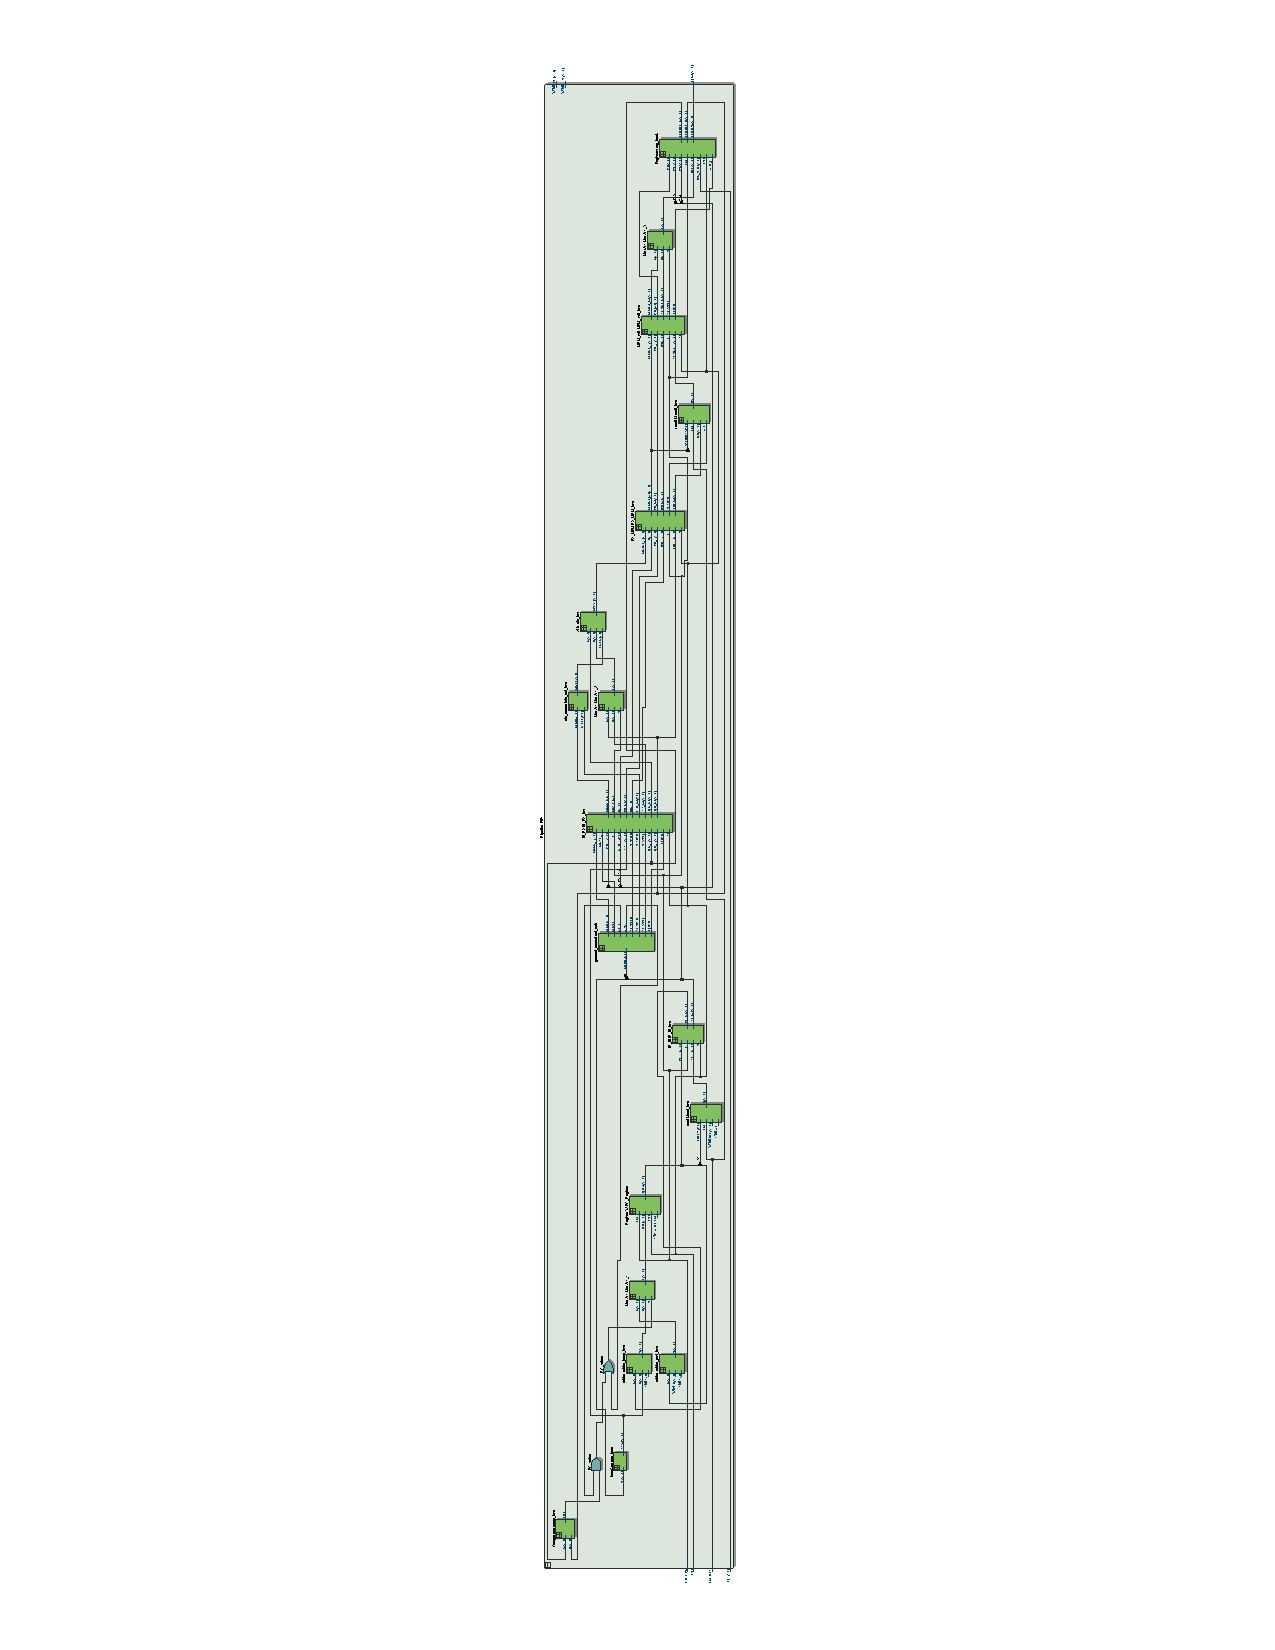
\includegraphics[
        trim=90mm 11mm 90mm 11mm,
        clip,
        angle=270,
        width=1\textwidth
    ]{Recursos/PDF/pipeline_rtl_view.pdf}
    \caption{Netlist RTL view do processador pipeline}
\end{figure}

\newpage

\paragraph{(b)} Compilando o projeto no Quartus, os requisitos físicos encontrados foram: 3.625 elementos lógicos; 1.349 registradores; 108 pinos; e memória total de 65.536 bits.

Ademais, a partir da análise temporal, encontramos os seguintes requisitos temporais: \textit{slack} de setup de 1,587 ns; \textit{slack} de \textit{hold} de 2,784 ns.

\paragraph{(c)} As simulações em forma de onda com o programa \cod{de1.s}, funcional e temporal, respectivamente, com frequência de 25 MHz são as das imagens a seguir:

\begin{figure}[H]
    \centering
    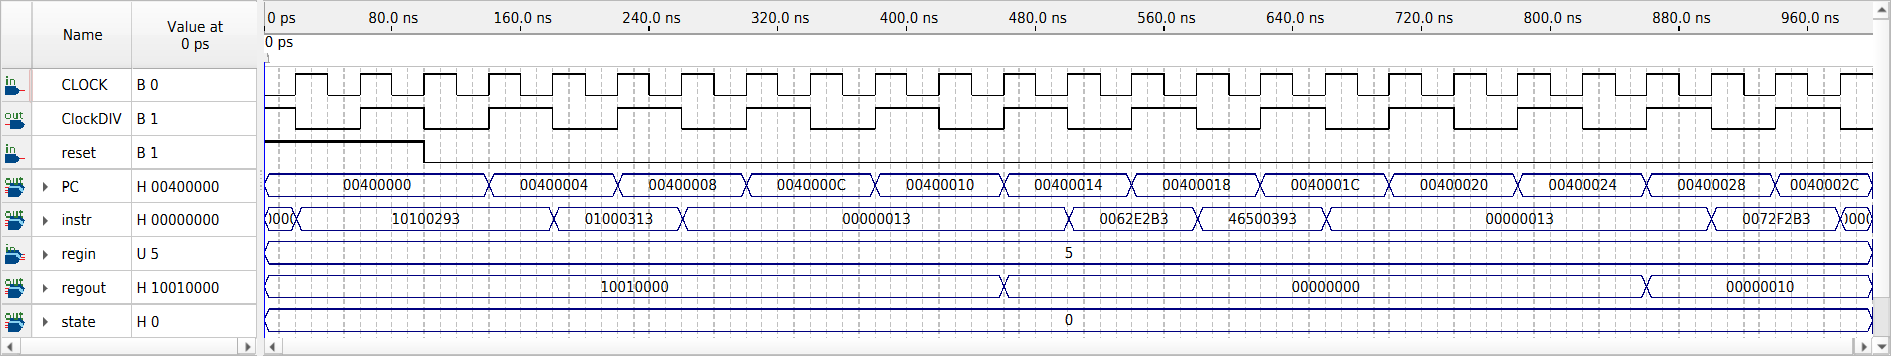
\includegraphics[width=\textwidth]{Recursos/Imagens/waveform_funcional.png}
    \caption{Forma de onda da simulação funcional}
\end{figure}

\begin{figure}[H]
    \centering
    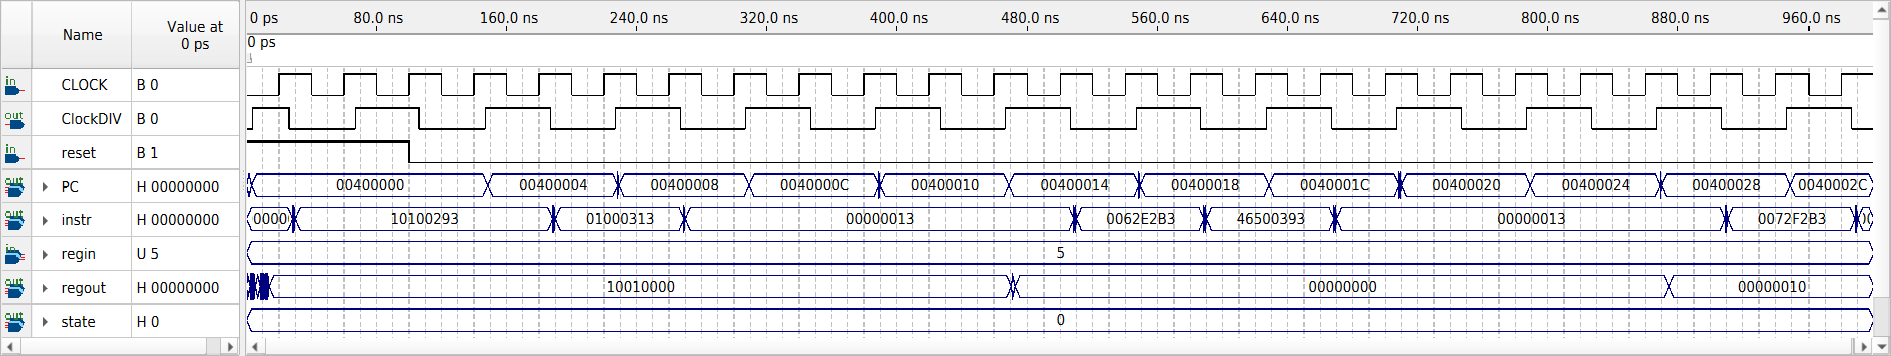
\includegraphics[width=\textwidth]{Recursos/Imagens/waveform_temporal.png}
    \caption{Forma de onda da simulação temporal}
\end{figure}

\paragraph{(d)} A frequência máxima encontrada pelo Quartus foi de 293 MHz (aproximadamente, 3,41 ns de período), mas essa frequência é limitada a 250 MHz devido ao período mínimo que o dispositivo físico aguenta. Simulando o processador com o código \cod{de1.s} e o período de clock de 4 ns, a forma de onda encontrada foi a da figura a seguir.

\begin{figure}[H]
    \centering
    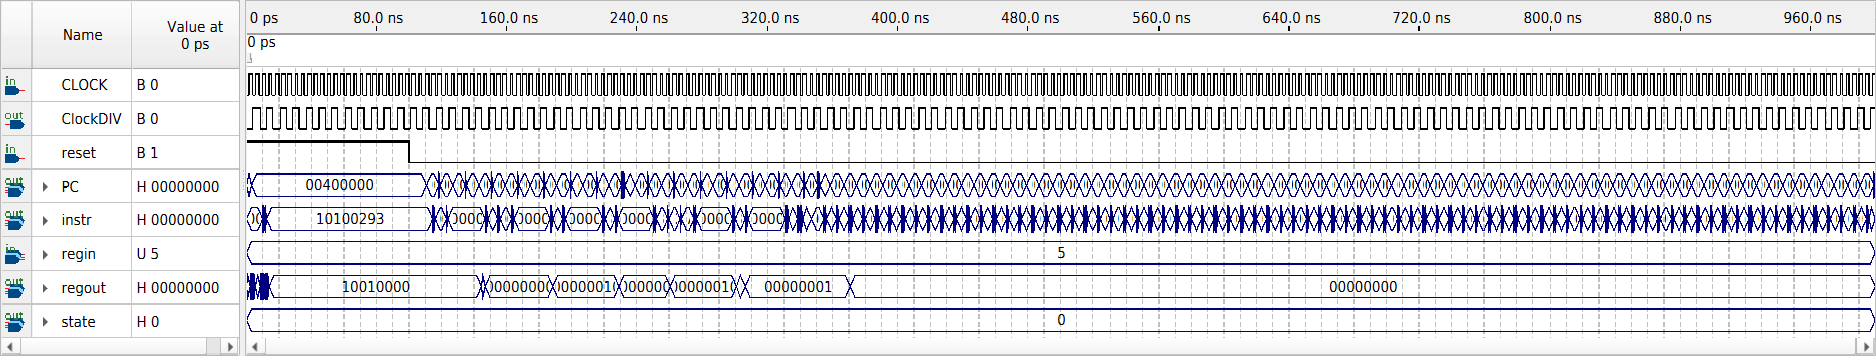
\includegraphics[width=\textwidth]{Recursos/Imagens/waveform_max_clock.png}
    \caption{Forma de onda da simulação com frequência máxima}
\end{figure}

Aparentemente, a frequência máxima calculada pelo Quartus, de fato, é realizável - pelo menos em simulação. Apesar de não ser possível visualizar com exatidão os valores do PC e da instrução, o valor do \cod{regout} é coerente, apontando o correto funcionamento do processador sob essa frequência.

\subsubsection{Tarefa III}
\begin{tcolorbox}[title=Enunciado, colback=blue!5!white, colframe=blue!75!black]
    Compare os requerimentos físicos e temporais dos seus 3 processadores (Uniciclo, Multiciclo e Pipeline). Comente. 
\end{tcolorbox}

Para realizar uma comparação mais precisa dos requerimentos físicos e temporais dos 3 processadores feitos nos projetos, será apresentada uma tabela comparativa a seguir:

\begin{table}[h!]
\centering
\resizebox{\textwidth}{!}{
\begin{tabular}{|c|c|c|c|c|c|c|c|}
\hline
\diagbox[width=4cm]{Processadores}{Requisitos} 
    & Elementos lógicos 
    & Registradores 
    & Pinos 
    & Bits de memória 
    & Setup (ns) 
    & Hold (ns) 
    & Frequência \\
\hline
Uniciclo 
    & \num{2642} 
    & \num{1025} 
    & \num{108} 
    & \num{65536} 
    & \num{5.982}
    & \num{4.293}
    & 71,34 MHz \\
\hline
Multiciclo 
    & \num{3291} 
    & \num{1253} 
    & \num{108} 
    & \num{65536} 
    & \num{6.690}
    & \num{2.715}
    & 302,11 MHz \\
\hline
Pipeline 
    & \num{2661} 
    & \num{1285} 
    & \num{108} 
    & \num{65536} 
    & \num{1.587}
    & \num{2.784}
    & 293,01 MHz \\
\hline
\end{tabular}
}
\end{table}

Ao analisar cada requerimento, primeiramente, é possível notar que a quantidade de elementos lógicos é praticamente igual entre os processadores uniciclo e pipeline, enquanto é maior no processador multiciclo. Isso se deve ao fato de que o pipeline, fundamentalmente, é bem parecido com o uniciclo, já que a ideia inicial do pipeline é dividir o uniciclo em etapas que operam concomitantemente. Além disso, o multiciclo utiliza mais elementos lógicos pois seu bloco de controle é mais complexo, possuindo mais sinais de saídas que os outros processadores e, também, em sua estrutura, estão presentes mais multiplexadores.

A quantidade de registradores é praticamente igual entre os processadores multiciclo e pipeline, enquanto é menor no processador uniciclo. Dessa forma, o pipeline utiliza mais registradores devido aos registradores de pipeline, que são fundamentais e únicos nos processos dessa CPU. O multiciclo, por sua vez, utiliza mais registradores devido ao seu bloco de controle, que funciona como uma máquina de estados finita e, também, devido à implementação de alguns registradores adicionais como: \cod{PCBack}, saídas \cod{A} e \cod{B} do banco de registradores e \cod{ALUOut}.

A quantidade de pinos e de bits de memória utilizados é idêntica nos 3 processadores. Isso acontece pelo fato de que eles rodam o mesmo programa, ou seja, a nível de software, realizam as mesmas operações.

Por último, também é extremamente importante tecer comentários sobre a frequência dos processadores. Seguindo esse prisma, é fácil observar que as frequências do multiciclo e do pipeline são bem maiores que a frequência do uniciclo. Isso faz perfeito sentido, já que tanto o multiciclo quanto o pipeline dividem as instruções em etapas menores, fazendo com que o tempo de clock seja baseado na etapa mais lenta, ao contrário do tempo de clock do uniciclo, que é baseado na instrução mais lenta. Assim, fica evidente o motivo de todos os processadores modernos serem baseados em pipeline, pois o pipeline consegue ter uma frequência bem alta ao dividir as instruções em pequenas etapas e, além disso, o pipeline também consegue ter uma CPI bem baixa, pois ele processa mais de uma instrução de cada vez, sem esperar que uma instrução termine antes de começar a próxima.



\subsubsection{Tarefa IV}
\begin{tcolorbox}[title=Enunciado, colback=blue!5!white, colframe=blue!75!black]
    Qual o melhor tempo que cada processador executa o programa \cod{de1.s}? Qual a explicação? 
\end{tcolorbox}

A fim de calcular o melhor tempo que cada processador utiliza para executar o programa \cod{de1.s}, é de praxe lembrar a equação característica que define o tempo de execução de cada programa, em que $\mathrm{I}$ se refere a quantidade de instruções, CPI se refere à quantidade média de ciclos para a execução de uma instrução e $\mathrm{T}_{\mathrm{clock}}$ é o período (nesse caso o máximo possível) para a execução do processador:
\begin{equation*}
    \mathrm{t}_{\mathrm{exec}} = \mathrm{I} \times \mathrm{CPI} \times \mathrm{T}_{\mathrm{clock}}
\end{equation*}

No caso do uniciclo, considerando que o programa, de acordo com o contador de instruções do próprio \textit{Rars}, executa 17 instruções, que o CPI dele é sempre 1 e que o período, de acordo com a frequência max (71,34 MHz), é de cerca de 14,017 ns. Obtendo, assim, 238,289 ns de tempo de execução.

Já para o caso do multiciclo a quantidade de instruções permanece e a frequência utilizada também é a máxima (302,11 MHz, o então 3,31 ns), contudo, o CPI utilizado é o médio, para tal devemos considerar os tipos de instruções e a quantidade de ciclos que cada uma demora para executar, assim como disponibilizado pela tabela com os dados fornecidos:

\begin{table}[H]
    \centering
\begin{tabular}{c|c|c|c}
Tipo de Instruções & Quantidade de Instruções & \% relativa & Ciclos necessários \\ \hline
Tipo R             & 6                        & 35          & 4                  \\
Tipo I             & 7                        & 41          & 5                  \\
Tipo S             & 1                        & 5           & 4                  \\
Tipo B             & 1                        & 5           & 3                  \\
Tipo J             & 2                        & 11          & 3                  
\end{tabular}
\end{table}

Dessa forma, obtêm-se um CPI de 4,13 instruções/clock. Sendo assim, o resultado do tempo de execução total é de cerca de 232,395 ns.

Por fim, no caso do pipeline, pela inserção de \cod{nop} como forma de evitar os hazards, a quantidade de instruções N foi alterada, obtendo 33 instruções ao todo, o CPI utilizado também é 1 e a frequência utilizada é a máxima (293,01 MHz,ou 3,41 ns de período). Assim, obtendo 112,53 ns de execução.


Todos os códigos desenvolvidos para a realização desse laboratório foram enviados compactados em um arquivo \cod{.zip}. Para acessar o vídeo solicitado, \href{https://www.youtube.com/watch?v=x1JfjiayK7M}{clique aqui}.
\end{document}